\documentclass[11pt,a4paper]{article}
\usepackage[utf8]{inputenc}
\usepackage[czech]{babel}
\usepackage[T1]{fontenc}
\usepackage{amsmath}
\usepackage{amsfonts}
\usepackage{amssymb}
\usepackage[total={18.5cm, 25cm}, top=1cm, bottom=0.5cm, left=1.25cm, includehead]{geometry}
\usepackage{fancyhdr} %záhlaví
\usepackage{float} % H aby neuplavali
\usepackage{pdfpages}


\usepackage{listings}
\usepackage{color}
 
\definecolor{codegreen}{rgb}{0,0.6,0}
\definecolor{codegray}{rgb}{0.5,0.5,0.5}
\definecolor{codepurple}{rgb}{0.58,0,0.82}
\definecolor{backcolour}{rgb}{0.95,0.95,0.92}
 
\lstdefinestyle{mystyle}{
    backgroundcolor=\color{backcolour},   
    commentstyle=\color{codegreen},
    keywordstyle=\color{magenta},
    numberstyle=\tiny\color{codegray},
    stringstyle=\color{codepurple},
    basicstyle=\footnotesize,
    breakatwhitespace=false,         
    breaklines=true,                 
    captionpos=b,                    
    keepspaces=true,                 
    numbers=left,                    
    numbersep=5pt,                  
    showspaces=false,                
    showstringspaces=false,
    showtabs=false,                  
    tabsize=2
}
 
\lstset{style=mystyle}



\pagestyle{fancy}
\fancyhf{}
% jednostranná sazba
\fancyhead[L]{
	%\begin{tabular}{lr}
	%	\textsc{Jan Vykydal} \\ 
	%	186240 
	%\end{tabular}
	\begin{minipage}{1.7cm}
		
\includegraphics[width=\textwidth]{../img/logo.pdf}
	\end{minipage}
}
\fancyhead[C]{
	\begin{tabular}{c}
		\textsc{Návod k sestavení} \\
		\textsc{Elektronické Kostky}
	\end{tabular} 
}
\fancyhead[R]{
	\begin{tabular}{lr}
		\multicolumn{2}{r}{FEKT UREL} \\
		\textsc{List:} & \thepage/\pageref{konec} 
	\end{tabular} 
}


\author{Jan Vykydal}
\title{Elektronická kostka}
\begin{document}

	
	\begin{figure}[H]
  \centering
  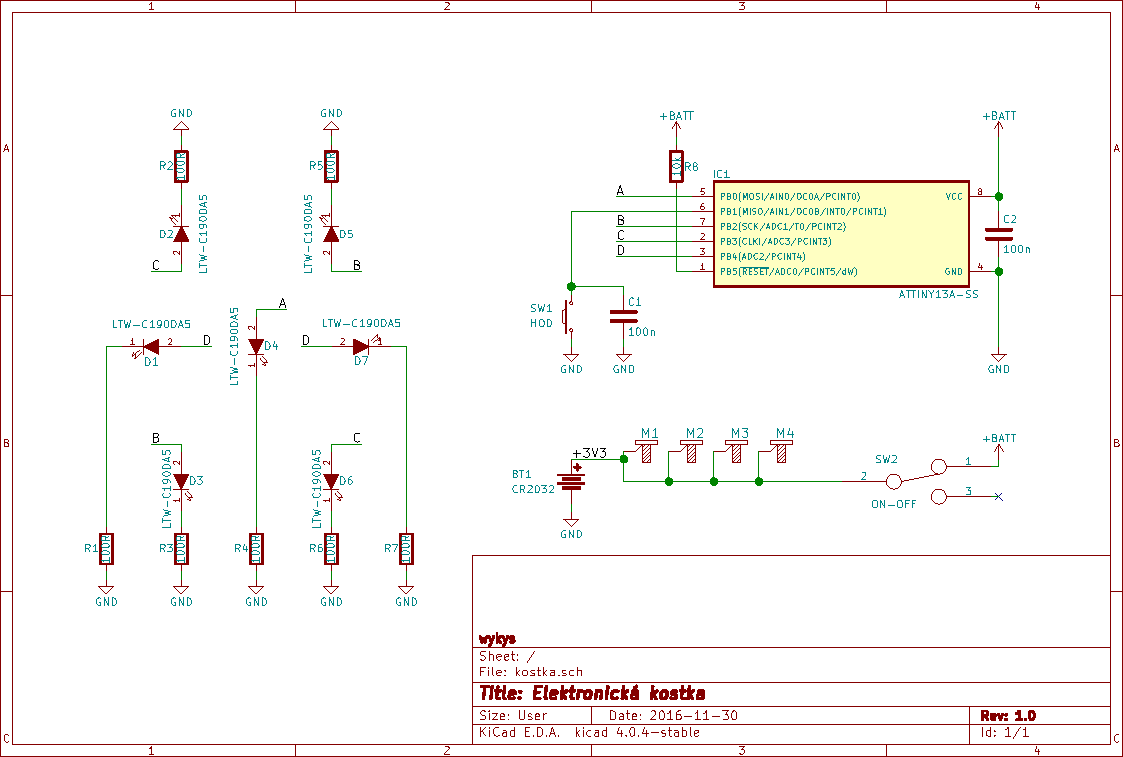
\includegraphics[width=\textwidth]{../design/sch_doc.pdf}
  \caption{Schéma zapojení}
  \label{img:1}
\end{figure}
  
  
\begin{table}[H]
  \begin{center}
    \begin{tabular}{c c}
      \begin{minipage}{0.48\textwidth}
        \begin{figure}[H]
          \centering
          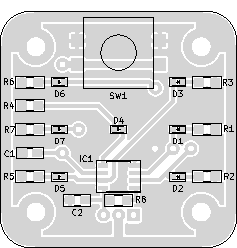
\includegraphics[width=\textwidth]{../design/svg/osazovak_top.pdf}
          \caption{Osazovací plán strana součástek}
          \label{img:2}
        \end{figure}
      \end{minipage}
  			&  				
      \begin{minipage}{0.48\textwidth}
        \begin{figure}[H]
          \centering
          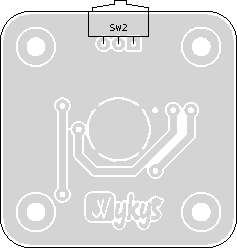
\includegraphics[width=\textwidth]{../design/svg/osazovak_bot.pdf}
          \caption{Osazovací plán strana spojů}
          \label{img:3}
        \end{figure}
      \end{minipage}
    \end{tabular}
  \end{center}	
\end{table}


\begin{table}[H]
  \begin{center}
    \begin{tabular}{c c}
      \begin{minipage}{0.48\textwidth}
        \begin{figure}[H]
          \centering
          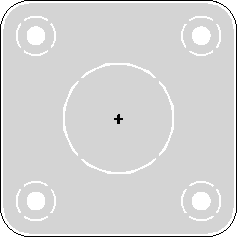
\includegraphics[width=\textwidth]{../design/svg/osazovak_spodek.pdf}
          \caption{Spodní destička, slouží jako přívod kladného pólu baterie k hlavní desce}
          \label{img:4}
        \end{figure}
      \end{minipage}
  			&  				
      \begin{minipage}{0.48\textwidth}
        \begin{table}[H]
        	\centering
        	\caption{Seznam součástek}
        	\vspace{5mm}
        	\begin{tabular}{c | c | c}
        		$R_1 - R_7$ & $100~\Omega$ & rezistor \\\hline
        		$R_8$ & $10~k\Omega$ & rezistor \\\hline
        		$C_1$, $C_2$ & $100~nF$ & kondenzátor \\\hline
        		$D_1 - D_7$ & LTW-C190DA5 & LED \\\hline
        		$IC_1$ & ATTINY13A-SSU & mikrokontorlér \\\hline
        		$SW_1$ & B3FS-4002P & tlačítko \\\hline
        		$SW_2$ & ESP2010 & přepínač \\\hline
        		$BT_1$ & CR2032 & baterie \\\hline
        		$M_1 - M_4$ & $2\cdot$ šroub a sloupek M3  & mechanické díly
        	\end{tabular}
        \end{table}
      \end{minipage}
      \\
      \begin{minipage}{0.48\textwidth}
        \begin{figure}[H]
          \centering
          \includegraphics[width=\textwidth]{../img/bila.png}
          \caption{ukázka uložení distančních sloupků a baterie CR2032}
          \label{img:6}
        \end{figure}
      \end{minipage}
  			&  				
      \begin{minipage}{0.48\textwidth}
        \begin{figure}[H]
          \centering
          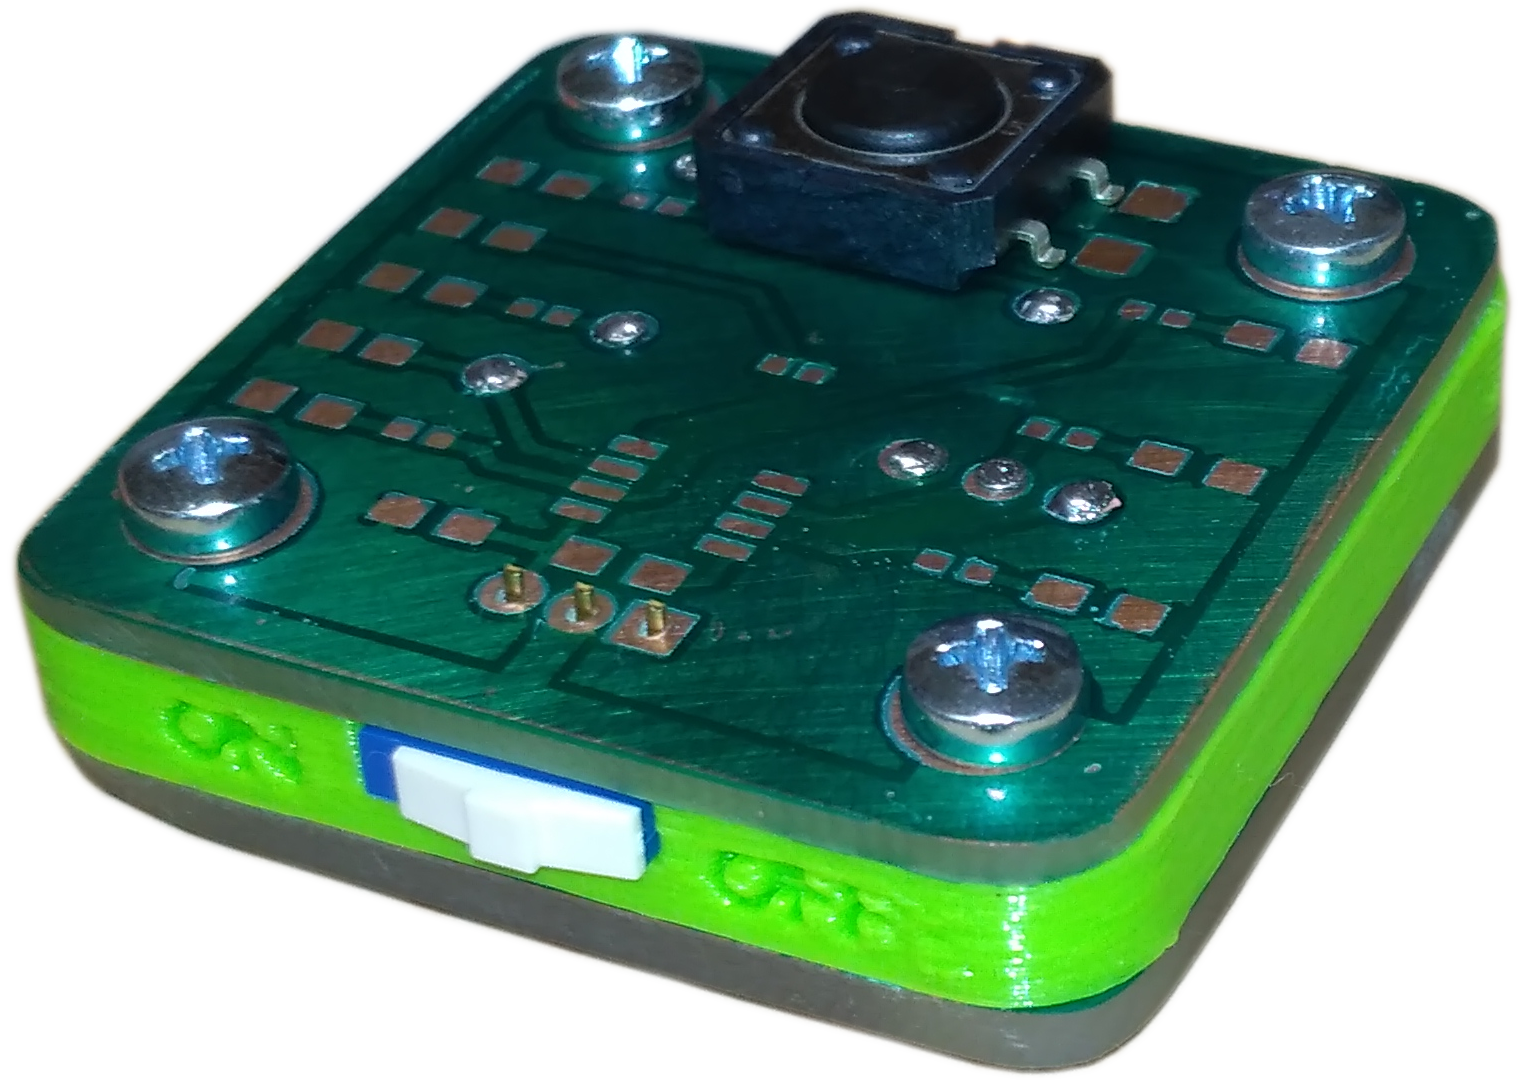
\includegraphics[width=\textwidth]{../img/zelena.png}
          \caption{smontovaná kostka bez osazených součástek}
          \label{img:7}
        \end{figure}
      \end{minipage}
    \end{tabular}
  \end{center}	
\end{table}

	
	\section*{Osazování}

Osazování je nejlepší provádět od nejmenších součástek po ty největší. Je tedy vhodné napřed osadit LED diody v pouzdře 0603, poté rezistory a kondenzátory v pouzdrech 0805. Následně mikrokontrolér v pouzdře SO-8 a nakonec tlačítko. Vypínač je vhodné přiletovat až když je kostka smontovaná, tak aby dobře pasoval do předchystaného otvoru.

Pozor na správnou polarizaci LED diod! Dioda je polarizovaná součástka, která má anodu a katodu. Katoda je označena malým kolečkem z horní strany a zelenou značkou ze strany spodní. Pokud budou diody nesprávně otočeny nebudou svítit. Správně osadit je třeba i mikrokontrolér, který při nevhodném osazení shoří. V osazovacím plánu je jednička mikrokontroléru označena čárkou. Poslední věcí, na kterou je třeba dávat obzvláště pozor je správné otočení baterie. Kladný pól, ten větší na, kterém je napsáno obvykle +, musí být položen na velkou plošku, spodní destičky, na které nejsou součástky. Záporný pól, ten menší je třeba připojit k malé plošce, která je na straně spojů hlavní destičky. Při špatném vložení baterie bude kostka zničena! Tak hodně štěstí.

\begin{figure}[H]
  \centering
  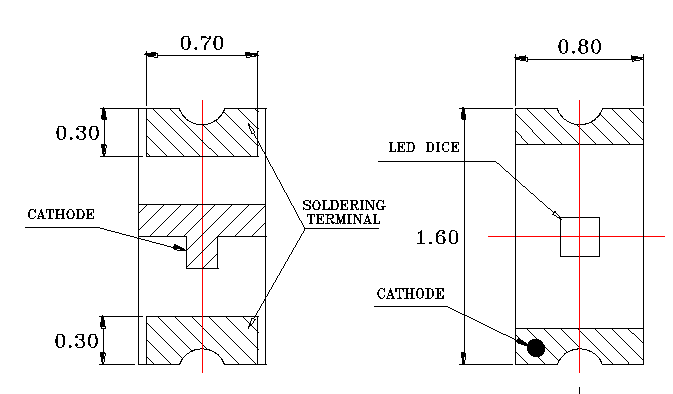
\includegraphics[width=\textwidth]{../img/LED.pdf}
  \caption{Označení katody LED diody LTW-C190DA5}
  \label{img:1}
\end{figure}
	\section*{Jak to funguje?}

Srdcem kostky je maličký mikrokontrolér ATTINY13, což je osmibitový čip s architekturou AVR. Jeho větší bratříčky lze nalézt třeba v ARDUINu. Mikrokontrolér nastaví svůj interní čítač tak, aby čítal od nuly do pětky. Dále nastaví přerušení na sestupnou hranu, které nastane při stisku tlačítka. Poté co vše nastaví, tak skočí do nekonečného cyklu.

Když je stisknuto tlačítko, tak nastane přerušení. Program je přerušen a po uložení adresy s programového čítače (to je místo kde se v programu právě nacházíme) do zásobníku (což je paměť typu Last In Last Out) skočí na obslužný podprogram přerušení. Dokud je tlačítko stisknuto, tak je na výstupních pinech generováno napětí takovým způsobem, který způsobuje postupné rozsvěcování LED a vyvolává efekt, že se točí.

Po uvolnění tlačítka je s registru čítače vyzvednuta aktuální hodnota. Tato hodnota se dekóduje pomocí tabulky a rozsvítí se příslušné LED, které zobrazí výslední číslo. Při zobrazování čísla ještě číslo třikrát zabliká, během doby kdy bliká nejde losovat další číslo. To je kvůli omezení podvádění několika rychlými stisky za sebou.

Když skončí podprogram přerušení, tak je ze zásobníku opět vyzvednuta adresa a program se opět vrátí do nekoneční smyčky.

Rezistory $R_1 - R_7$ tu jsou kvůli nastavení pracovního bodu LED diody. Bez nich by LED shořely. Rezistor $R_8$ tu je kvůli nastavení vhodné úrovně na RESETu. Bez něj by se zařízení mohlo restartovat. Kondenzátor $C_1$ slouží k eliminaci kmitů napětí při stisku či uvolnění tlačítka. Kondenzátor $C_2$ tu je kvůli odfiltrování rušení a možnosti v případě potřeby poskytnout mikrokontroléru krátkodobě potřebný proud.
	\section*{Zdrojový kód}

\lstset{
  language=C,                	  % choose the language of the code
  numbers=left,                   % where to put the line-numbers
  stepnumber=1,                   % the step between two line-numbers.        
  numbersep=5pt,                  % how far the line-numbers are from the code
  backgroundcolor=\color{white},  % choose the background color. You must add \usepackage{color}
  showspaces=false,               % show spaces adding particular underscores
  showstringspaces=false,         % underline spaces within strings
  showtabs=false,                 % show tabs within strings adding particular underscores
  tabsize=2,                      % sets default tabsize to 2 spaces
  captionpos=b,                   % sets the caption-position to bottom
  breaklines=true,                % sets automatic line breaking
  breakatwhitespace=true,         % sets if automatic breaks should only happen at whitespace
  title=firmware kostky 08.12.2016,                 % show the filename of files included with \lstinputlisting;
}

\lstinputlisting{../fw/kostka/kostka/main.c}

	
	\label{konec}

\end{document}